\documentclass{article}
\usepackage[left=25mm,top=1.5in,bottom=0.8in]{geometry}
\usepackage{fancyhdr}
\usepackage{graphicx}
\usepackage{extramarks}
\usepackage{amsmath}
\usepackage{amsthm}
\usepackage{amsfonts}
\usepackage{tikz}
\usepackage[plain]{algorithm}
\usepackage{algpseudocode}
\usepackage{listings}
\graphicspath{ {./} }
\definecolor{codegreen}{rgb}{0,0.6,0}
\definecolor{codegray}{rgb}{0.5,0.5,0.5}
\definecolor{codepurple}{rgb}{0.58,0,0.82}
\definecolor{backcolour}{rgb}{0.95,0.95,0.92}

\lstdefinestyle{mystyle}{
    backgroundcolor=\color{backcolour},
    commentstyle=\color{codegreen},
    keywordstyle=\color{magenta},
    numberstyle=\tiny\color{codegray},
    stringstyle=\color{codepurple},
    basicstyle=\ttfamily\footnotesize,
    breakatwhitespace=false,         
    breaklines=true,                 
    captionpos=b,                    
    keepspaces=true,                 
    numbers=left,                    
    numbersep=5pt,                  
    showspaces=false,                
    showstringspaces=false,
    showtabs=false,                  
    tabsize=2
}
\pagestyle{fancy}
\lhead{Sambhrant Maurya}
\chead{CS 685}
\rhead{Assignment 1}
\cfoot{\thepage}

\title{CS 685 (Data Mining)
Assignment 1 \\ Report}
\author{\textbf{Sambhrant Maurya} \\ Roll No. 20111054}
\date{Due date: September 25, 2020 \\ Instructor: Prof. Arnab Bhattacharya}

\setcounter{secnumdepth}{0}
\newcounter{partCounter}

\begin{document}

\maketitle
\pagebreak
\lstset{style=mystyle}
\section{Analysis of mined data}
\subsection{Trend of COVID-19 cases in India with time}
It can be observed that the number of COVID-19 cases in India have been on exponential rise from the month of March. Metropolitan towns of India- Delhi and Mumbai show this trend very clearly. The image below (taken from cases-months.csv) shows this trend for Delhi. Cases have risen exponentially till the month of June after which there has been a slight fall in the number of cases for the next three months. 
\begin{figure}[h]
\centerline{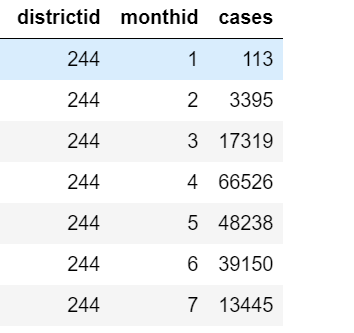
\includegraphics{delhi_month.png}}
\caption{Monthly COVID-19 cases in Delhi}
\label{fig}
\end{figure} \\
While the number of monthly cases in Delhi have seen a fall in the last two months, other towns like Bangalore have not been so lucky. Below is a series (taken from cases-month.csv) showing the rise in the number of COVID-19 cases in the district Bangalore Urban. \\
\begin{figure}[htbp]
\centerline{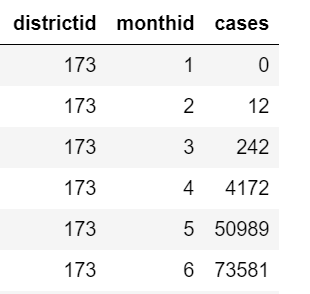
\includegraphics{bangalore.png}}
\caption{Monthly COVID-19 cases in Bangalore}
\label{fig}
\end{figure} \\
It can be seen that the number of cases in Bangalore is still on a sharp rise and Bangalore now has more number of cases than Delhi. A similar conclusion can be drawn for other metropolitan cities in India- Kolkata, Chennai and Pune, which are emerging as the new hotspots in the recent months. \\
However, it should also be noted that the number of cases in these districts is in tally with the population in these districts. As much of India's population is concentrated in these districts, the number of COVID-19 cases is also high in these districts.\\
Taking an example of a smaller Indian district like Mirzapur, UP it can be seen that the number of cases has been on the gradual rise in this district too.\\
\begin{figure}[h]
\centerline{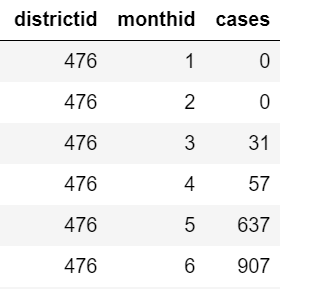
\includegraphics{mirzapurmonthly.png}}
\caption{District Mirzapur,UP-monthly cases}
\label{fig}
\end{figure} \\
The overall analysis below (taken from cases-overall.csv) shows that these 5 districts have the most number of COVID-19 cases from 15 March, 2020 to 5 September, 2020.
\begin{figure}[h]
\centerline{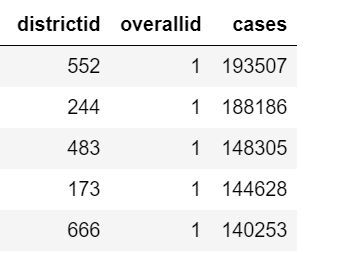
\includegraphics{overallcases.png}}
\caption{Top 5 districts with the highest number of COVID cases}
\label{fig}
\end{figure} \\
\\
\\
It can be seen that the districts- \textit{Pune-552}, \textit{Delhi-244},\textit{Mumbai-483},\textit{Bengaluru Urban-173} and \textit{Thane-666} had the most number of COVID-19 cases in the mentioned time period. \\
The series below(taken from top-overall.csv) shows the top 5 hotspots and coldspots in the country when the number of cases in a district is compared with the number of cases in it's neighbors and the state as a whole. \\
\begin{figure}[h]
\centerline{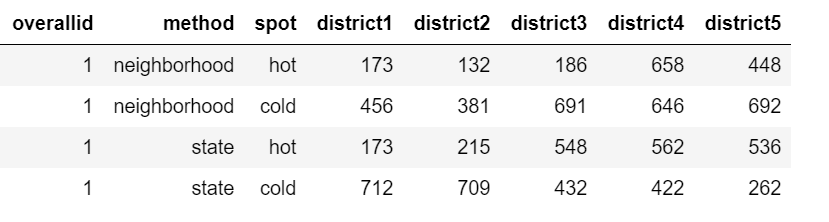
\includegraphics{hotspotsoverall.png}}
\caption{Top 5 hotspots and coldspots in the mentioned time period}
\label{fig}
\end{figure} \\
On analyzing the data from top-month.csv, it can be observed that the top hotspot and coldspot districts for different months changes quite unpredictably. Districts in Mumbai were the hotspots in the months of March-June, however June onwards, the trend shifted, making other districs like Bangalore Urban (district id 173) and Telangana districts (district id 665) the hotspots. 
\section{Conclusion}
The mined data is very useful to analyze the behavior of the COVID-19 crisis in India for the \textbf{past}. The data can be used to obtain the weekly/monthly and overall number of COVID-19 cases in the given time period and hence it can also be used to obtain the hotspots and coldspots in the country. \\
\\
However, the mined data fails to provide any predictions for the \textbf{future} of the pandemic. This can be attributed to the unpredictable nature of the COVID-19 crisis in India-the growth in number of cases has not followed any predictable trend and it's very difficult to predict which districts will become the hotspots in the future and when the COVID-19 crisis will come to an end .
\end{document}
